\part{Entrega 0}

Actualmente, el análisis de estructuras se realiza computacionalmente. Esto no solo ayuda a realizar los cálculos más rápido, sino que también permite llevar a cabo múltiples diseños en un corto período de tiempo. Esta sección tiene como objetivo aprender sobre la librería OpenSees y el análisis que hay detrás de un reticulado. Para esto, se realizó un análisis manual y se comparó con el análisis realizado en OpenSees.
\\ \\
El reticulado de referencia es el siguiente:

\begin{figure}[H]
    \centering
    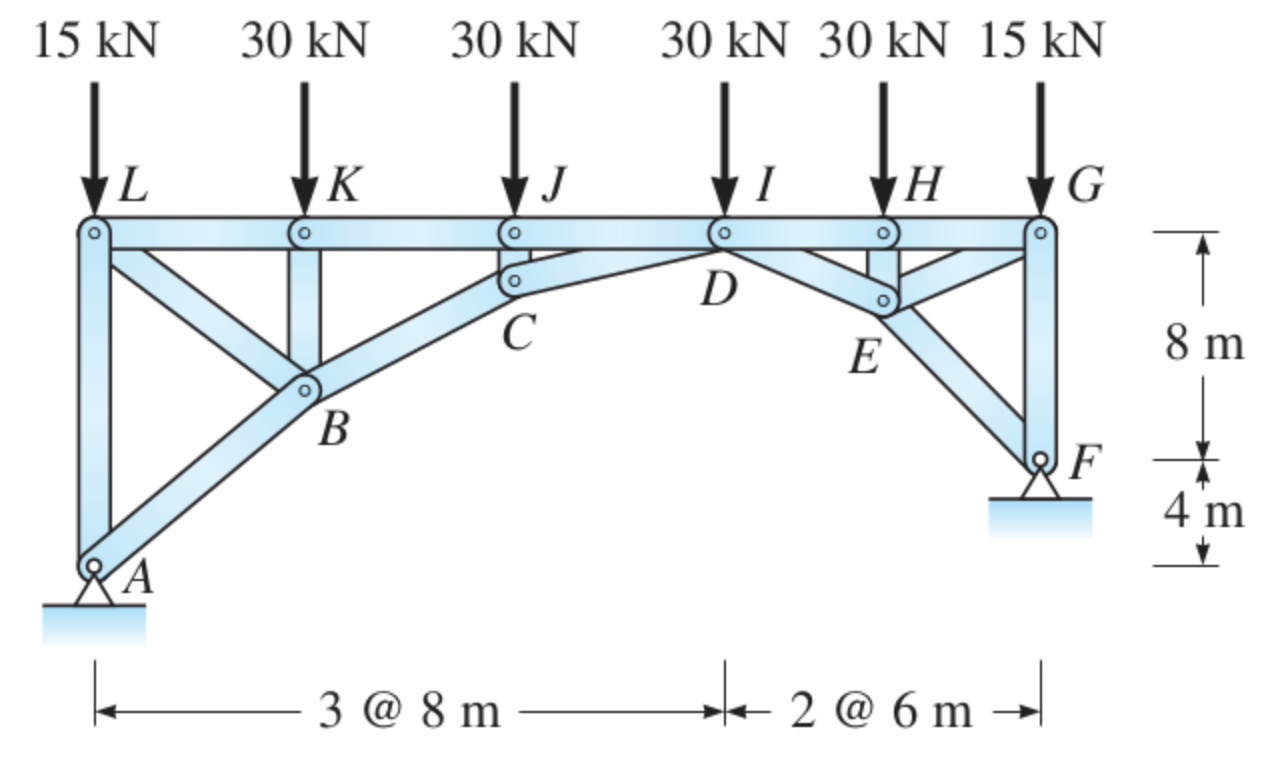
\includegraphics[width=0.7\textwidth]{FOTOS/reticulado.png}
    \caption{Reticulado}
    \label{fig:reticulado}
\end{figure}

\section{Material Utilizado}

Para el cálculo de deformaciones, se consideró un módulo de elasticidad de 200 GPa y una fluencia de 210 MPa. Además, el mínimo factor de seguridad aceptado fue determinado en 1.3.

\section{Comandos Para Correr Arquitectura X86 en Arquitectura ARM}

Dado que trabajo en Mac, la arquitectura utilizada es ARM64, mientras que el requerimiento para las librerías es X86. Por lo tanto, se debe correr una instancia de X86 en la arquitectura ARM. Para activar el entorno, se utilizan los siguientes comandos:

Primero, se llama la instancia en una arquitectura X86:

\begin{verbatim}
    arch -x86_64 python3 -m venv x86_env
\end{verbatim}

Luego, se activa:

\begin{verbatim}
    source x86_env/bin/activate
\end{verbatim}

Para instalar las librerías necesarias:

\begin{verbatim}
    arch -x86_64 pip install <librerías>
\end{verbatim}

Finalmente, se debe correr el código desde la instancia:

\begin{verbatim}
    arch -x86_64 python3 <ruta>.py
\end{verbatim}

\section{Cálculos Manuales}

\subsection{Cálculo de alturas}

Para calcular la altura de los puntos desconocidos, se determinó el momento en tal nodo, obteniendo así:

\begin{table}[H]
    \centering
    \begin{tabular}{|c|c|}
    \hline
    \textbf{Nodo} & \textbf{Altura [m]}  \\ 
    \hline
    B & 7.733  \\ 
    C & 11.733  \\ 
    E & 9.400 \\ 
    \hline
    \end{tabular}
    \caption{Alturas Nodos Desconocidos}
\end{table}

\subsection{Solución Reticulado}

El código realizado para calcular el reticulado se encuentra en el \href{https://github.com/LukasWolff2002/PROYECTO_3_MCOC/blob/main/CODIGO/CODIGO_MANUAL/solucion_reticulado.py}{siguiente enlace}, y para calcular la sección de las barras, se utilizó el \href{https://github.com/LukasWolff2002/PROYECTO_3_MCOC/blob/main/CODIGO/CODIGO_MANUAL/tipo_barras.py}{siguiente código}.

\begin{table}[H]
    \centering
    \begin{tabular}{|c|c|c|c|c|}
    \hline
    \textbf{Barra} & \textbf{Esfuerzo Interno} & \textbf{D$_{int}$, D$_{ext}$ [mm]} & \textbf{Tensiones Internas} & \textbf{Fuerza Crítica Pandeo} \\ 
    \hline
    AB & 89.411 & (117.000, 135.500) & 24.371 & 117.169 \\ 
    AL & 15.000 & (85.000, 95.000) & 10.610 & 19.682 \\ 
    LK & 0.000 & (10.000, 20.000) & 0.000 & 0.227 \\ 
    LB & 0.000 & (10.000, 20.000) & 0.000 & 0.177 \\ 
    BC & 71.874 & (98.500, 114.500) & 26.852 & 94.163 \\ 
    BK & 30.000 & (52.000, 62.000) & 33.506 & 39.731 \\ 
    KJ & 0.000 & (10.000, 20.000) & 0.000 & 0.227 \\ 
    JC & 30.000 & (10.000, 20.000) & 127.324 & 204.387 \\ 
    JI & 0.000 & (10.000, 20.000) & 0.000 & 0.227 \\ 
    CI & 64.321 & (90.000, 105.000) & 27.999 & 84.599 \\ 
    IH & 0.000 & (10.000, 20.000) & 0.000 & 0.404 \\ 
    IE & 70.062 & (77.500, 93.500) & 32.604 & 91.438 \\ 
    HE & 30.000 & (36.000, 46.000) & 46.582 & 40.103 \\ 
    HG & 0.000 & (10.000, 20.000) & 0.000 & 0.404 \\ 
    GE & 0.000 & (10.000, 20.000) & 0.000 & 0.340 \\ 
    GF & 15.000 & (63.500, 73.500) & 13.941 & 19.569 \\ 
    EF & 86.488 & (92.500, 110.500) & 30.137 & 112.836 \\ 
    \hline
    \end{tabular}
    \caption{Información Barras}
\end{table}

\textbf{Nota:} Todas las barras se encuentran en esfuerzo de compresión.

\begin{table}[H]
\centering
\begin{tabular}{|c|c|c|}
\hline
\textbf{Barra} & \textbf{FS Fluencia} & \textbf{FS Pandeo} \\ 
\hline
AB & 8.617 & 1.310 \\ 
AL & 19.792 & 1.312 \\ 
BC & 7.821 & 1.310 \\ 
BK & 6.267 & 1.324 \\ 
JC & 1.649 & 6.813 \\ 
CI & 7.500 & 1.315 \\ 
IE & 6.441 & 1.305 \\ 
HE & 4.508 & 1.337 \\ 
GF & 15.064 & 1.305 \\ 
EF & 6.968 & 1.305 \\ 
\hline
\end{tabular}
\caption{Factor de Seguridad Fluencia y Pandeo}
\end{table}

\textbf{Nota:} Solo se consideran las barras que tienen algún esfuerzo interno significativo para el cálculo del FS.

\subsection{Cálculo de Deformación}

Para el cálculo de la deformación en el nodo D/I, se impone una fuerza virtual igual a 1. De esta manera, es posible calcular el reticulado. Con todos los esfuerzos conocidos, se aplica la siguiente fórmula:

\begin{equation}
    \delta = \sum   \frac{P_r \cdot P_v \cdot L}{E\cdot A}
\end{equation}

Se obtuvieron los siguientes desplazamientos, donde la sección considerada es (117, 135.5):

\begin{equation}
    \delta_x = -8.47300012321403 mm \quad \delta_y = -10.1170948633426 mm
\end{equation}

El código para calcular el desplazamiento horizontal está en el \href{https://github.com/LukasWolff2002/PROYECTO_3_MCOC/blob/main/CODIGO/CODIGO_MANUAL/desplazamiento_horizontal.py}{siguiente enlace}, mientras que el código para el desplazamiento vertical está en el \href{https://github.com/LukasWolff2002/PROYECTO_3_MCOC/blob/main/CODIGO/CODIGO_MANUAL/desplazamiento_vertical.py}{siguiente enlace}.

\section{OpenSees}

Para realizar el modelo en OpenSees, se agregó la barra KC, de modo que el sistema no fuera hiperestático. Aun así, esto no afectó el cálculo, ya que dicha barra no tiene esfuerzo interno considerable.

\subsection{Solución Reticulado}

El código utilizado para hacer el modelo en OpenSees se encuentra en el \href{https://github.com/LukasWolff2002/PROYECTO_3_MCOC/blob/main/CODIGO/OPENSEES/E0_Wolff.py}{siguiente enlace}, y los esfuerzos obtenidos son los siguientes:

\begin{table}[H]
    \centering
    \caption{Esfuerzos internos en las barras (fuerzas axiales)}
    \label{tab:esfuerzos_internos}
    \begin{tabular}{|c|c|}
        \hline
        \textbf{Barra} & \textbf{Fuerza Axial (KN)} \\
        \hline
        AL & 15.03 \\
        AB & 89.39 \\
        LB & 0.06  \\
        LK & 0.05  \\
        KB & 30.03 \\
        BC & 71.82 \\
        KJ & 0.79  \\
        KC & 0.74  \\
        JC & 30.00 \\
        CD & 63.53 \\
        JI & 0.79  \\
        IH & 0.00  \\
        IE & 70.06 \\
        HE & 30.00 \\
        EF & 0.00  \\
        HG & 0.00  \\
        EF & 86.49 \\
        GF & 15.00 \\ \hline
    \end{tabular}
\end{table}

\textbf{Nota:} Se observa claramente una relación directa con los resultados manuales, donde la pequeña variación nace de la adición de la barra \textbf{KC}.

\subsection{Deformaciones}

Para el cálculo de las deformaciones, se asume una sección igual para todas las barras. Según los datos calculados manualmente, la sección necesaria es (117, 135.5), y los resultados obtenidos son los siguientes:

\begin{figure}[H]
    \centering
    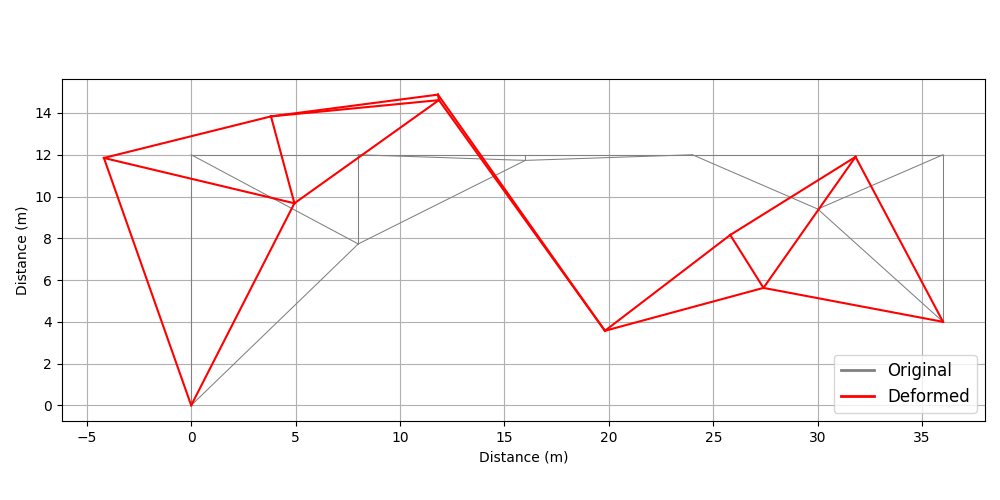
\includegraphics[width=0.7\textwidth]{GRAFICOS/deformed_truss.png}
    \caption{Deformaciones en los nodos}
    \label{fig:deformaciones}
\end{figure}

El diagrama tridimensional solicitado es el siguiente:

\begin{figure}[H]
    \centering
    \includegraphics[width=0.7\textwidth]{GRAFICOS/3D.png}
    \caption{Gráfico 3D}
    \label{fig:deformaciones_3D}
\end{figure}

La deformación observada en el nodo D/I es:

\begin{equation}
    \delta_x = -0.0065527383052691 m \quad \delta_y = -0.013182996668814742 m
\end{equation}

De esta manera, los porcentajes de error respecto al cálculo manual son:

\begin{equation}
    \delta_x = 29.31\% \quad \delta_y = 30.23\%
\end{equation}

\section{Conclusión}

En conclusión, los objetivos de la presente entrega fueron logrados correctamente. Se logró generar un análisis del reticulado de manera manual, donde se determinaron los distintos factores de seguridad, además de las secciones mínimas que debe tener cada barra. Tomando como referencia la barra de mayor área e inercia, se determinó el desplazamiento en el nodo solicitado mediante fuerzas virtuales.
\\ \\
Posteriormente, se realizó el mismo análisis en OpenSees, donde se observó que los resultados no variaron significativamente. Se determinó el desplazamiento en el nodo D y se generaron los gráficos solicitados.
\\ \\
Finalmente, se cuantificó el error entre ambos métodos, comparando la variación del desplazamiento calculado. Considerando las pequeñas variaciones en el cálculo, el error está dentro de un rango esperado.


\newpage
\section{Anexos}

El razonamiento utilizado para el código OpenSees es el siguiente:

\begin{lstlisting}[language=Python]
    # Se define un modelo 2D con 2 grados de libertad
    ops.wipe()
    ops.model('basic', '-ndm', 2, '-ndf', 2)
\end{lstlisting}

\begin{lstlisting}[language=Python]
    # Definir el material uniaxial elástico, con módulo de elasticidad E
    matTag = 1  # Material tag
    ops.uniaxialMaterial('Elastic', 1, E)
\end{lstlisting}

\begin{lstlisting}[language=Python]
    # Se definen los nodos
    nodes = {
    1: (0, 0),
    2: (0, 12),
    3: (8, 7.73),
    4: (8, 12),
    5: (16, 11.73),
    6: (16, 12),
    7: (24, 12),
    8: (30, 9.4),
    9: (30, 12),
    10: (36, 12),
    11: (36, 4)
    }
    # Generar los nodos
    for node_id, coords in nodes.items():
        ops.node(node_id, *coords)
\end{lstlisting}

\begin{lstlisting}[language=Python]
    # Definir los elementos truss
    elements = [
        (1, 2), #1
        (1, 3), #2BC
        (2, 3), #3
        (2, 4), #4
        (3, 4), #5
        (3, 5), #6
        (4, 6), #7
        (4, 5), #8
        (5, 6), #9
        (5, 7), #10
        (6, 7), #11
        (7, 9), #12
        (7, 8), #13
        (8, 9), #14
        (8, 10), #15
        (9, 10), #16
        (8, 11), #17
        (10, 11) #18
    ]

    for i, (ni, nj) in enumerate(elements, start=1):
        ops.element('Truss', i, ni, nj, A1, matTag)
\end{lstlisting}

\begin{lstlisting}[language=Python]
    # Se definen las restricciones
    ops.fix(1, 1, 1)  
    ops.fix(11, 1, 1)  
    # El nodo 1 y el nodo 11 son fijos en x e y
\end{lstlisting}

\begin{lstlisting}[language=Python]
    # Definir cargas en los nodos
    ops.timeSeries('Constant', 1)
    ops.pattern('Plain', 1, 1)
    ops.load(2, 0.0, -15000.0)
    ops.load(4, 0.0, -30000.0)
    ops.load(6, 0.0, -30000.0)
    ops.load(7, 0.0, -30000.0)
    ops.load(9, 0.0, -30000.0)
    ops.load(10, 0.0, -15000.0)
\end{lstlisting}

\begin{lstlisting}[language=Python]
    # Se resuelve el modelo
    ops.system('BandSPD')
    ops.numberer('RCM')
    ops.constraints('Plain')
    ops.integrator('LoadControl', 1.0)
    ops.algorithm('Linear')
    ops.analysis('Static')

    # Ejecutar análisis
    if ops.analyze(1) != 0:
        print("Error en el análisis estático")
    else:
        print("Análisis estático exitoso")
\end{lstlisting}
